
\lecture{Introduction}{Introduction}
\section{Introduction}

\title{Statistics}
\subtitle{Introduction and Section 2.1}

\author{Kelly Black}
\institute{Clarkson University}
\date{13 January 2012}

\begin{frame}
  \titlepage
\end{frame}

\begin{frame}
  \frametitle{Outline}
  \tableofcontents[pausesection,hideothersubsections,sectionstyle=show/hide]
\end{frame}


\section{Class Information}


\begin{frame}
  \frametitle{Class Information}

\begin{description}
\item[Textbook] {\em Elementary Statistics}, Eleventh Edition, by
  Johnson and Cuby, Brooks/Cole;. (ISBN 9780538733502) The book is
  available at the bookstore as well as many on-line outlets.

\end{description}

\end{frame}


\begin{frame}
  \frametitle{Class Information}

\begin{description}
\item[Grading] %~ \\ %\samepage
  
  The final grades are calculated using the following distribution:
    \begin{tabular}[t]{rl}
      40\% & Three Exams, \\
      20\% & Quizzes, \\
      20\% & Webworks, \\
      5\%  & Attendance/Clicker Response \\
      15\% & Final Exam.
    \end{tabular}
  
    At the end of the semester we assign letter grades as follows:
    90\% for an A, 86\% for a B+, 80\% for a B, 76\% for a C+, 70\%
    for a C, 66\% for a D+, and \%60 for a D.
\end{description}

\end{frame}



\begin{frame}
  \frametitle{Class Information}

\begin{description}
  \item[Exam Dates] The first test is tentatively scheduled for
    Monday, February 13, at 6:00pm in Science Center 360. The second
    test is tentatively scheduled for Friday, 9 March, at 6:00pm in
    Science Center 360 . The third test is tentatively scheduled for
    Monday, 16 April, at 6:00pm in Science Center 360.  You should
    bring your own pencils, blank paper, calculators, and good luck
    charms.  The professor will not have any spare materials.

 
\end{description}

\end{frame}

\begin{frame}
  \frametitle{Class Information}

\begin{description}
\item[Quiz] There will be a quiz every other week in class \textbf{and
    in your recitations}. The quizzes will be similar to the posted
  homework problems. The lowest quiz score will be dropped.
\end{description}

\end{frame}


\begin{frame}
  \frametitle{Class Information}

\begin{description}
  \item[Clickers] A portion of your grade is for classroom attendance
    and participation. This is measured using clickers. Each day one
    or more questions will be asked, and you will be asked to respond
    using the clicker. The clicker that we are using is from Turning
    Point Technologies, and we recommend that you use the ResponseCard
    RF LCD clicker. You can purchase the clicker at
    \url{https://store.turningtechnologies.com} The Clarkson
    University promotional code is Z0k0.

\end{description}

\end{frame}

\begin{frame}
  \frametitle{Class Information}

 Here is what you need to do to register your clicker:
\begin{enumerate}
\item Go to the website student.turningtechnologies.com
\item Enter your ResponseCard ID (found on back of unit)
\item Enter your first name and last name in the appropriate fields. 
\item Enter the name of your pet in the "Other Field" entry. If you do not have a pet then enter "none."
\item Complete the security entry
\item Press Next
\item Enter my email address, kblack@clarkson.edu 
\item Select the class name, STAT 282 - Spring 2012. 
\item Click Next and confirm information. 
\item You may click ``Back'' if you find information you need to correct.
\end{enumerate}

\end{frame}

\begin{frame}
  \frametitle{Class Information}

\begin{description}
  \item[Webwork] Webwork is a web based homework system. You can find
    it at the following URL: \\
    \url{http://black.sc.clarkson.edu/webwork2/}.
\end{description}

\end{frame}


\begin{frame}
  \frametitle{Class Information}

\begin{description}
  \item[Academic Accommodations] If you require any kind of special
    accommodation please come see me.  Requests for academic
    accommodations must be made during the first three weeks of the
    semester, except for unusual circumstances.  Students must
    register with the Office of Accommodative Services, located in the
    Student Success Center, 110 ERC, to verify their eligibility for
    appropriate accommodations.


\end{description}


\end{frame}

\begin{frame}
  \frametitle{Class Information}

\begin{description}
  \item[Office Hours] Monday, Wednesdays, and Fridays from 9:00am to
    11:00am, and Tuesdays from 10:00am to 12:00pm.  If you would like
    to meet at another time please contact me and arrange for a
    meeting.

\end{description}


\end{frame}

\section{Data (Fukushima Radiation Survey)}

\begin{frame}
  \frametitle{Data}

  Different kinds of data....

  Today just look at graphical views of data.

\end{frame}

\begin{frame}
  \frametitle{Example Data Set}

  Fukushima Radiation Survey

  Measurements taken during the 11 march 2011 crisis after the
  T\={o}hoku earthquake:
  \begin{itemize}
  \item Time
  \item Date
  \item Longitude
  \item Latitude
  \item Distance From Source
  \item Direction From Source
  \item Radiation Level (mRad/hour)
  \item Description
  \item several others
  \end{itemize}

\end{frame}



\begin{frame}
  \frametitle{Direction}

  \begin{tabular}{c}
    Direction \\ \hline 
    N   \\
    NNE  \\
    NNW  \\
    NW  \\
    S  \\
    SSW \\
    SW  \\
    W  \\
    WNW  \\
    WSW 
  \end{tabular}

\end{frame}

\begin{frame}
  \frametitle{Direction}

  \begin{tabular}{c|c}
    Direction & Number \\ \hline
    N  & 7 \\
    NNE & 6 \\
    NNW & 21 \\
    NW   & 45 \\
    S  & 13 \\
    SSW  & 484 \\
    SW   & 958 \\
    W & 118 \\
    WNW & 32 \\
    WSW & 218
  \end{tabular}

\end{frame}

\section{Graphical View of Data}

\begin{frame}
  \frametitle{Direction - Bar Chart}

  \begin{center}
    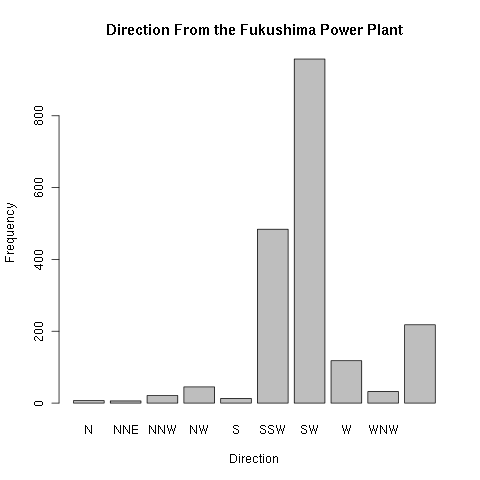
\includegraphics[width=8cm]{img/fukushimaDirectionBarPlot}
  \end{center}

\end{frame}

\begin{frame}
  \frametitle{Direction - Pareto Chart}

  \begin{center}
    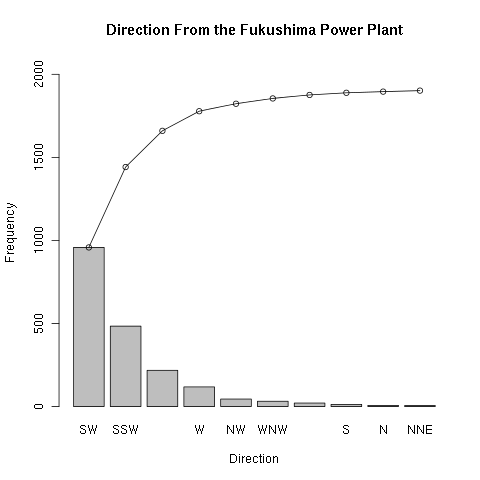
\includegraphics[width=8cm]{img/fukushimaParetoDirection}
  \end{center}

\end{frame}

\begin{frame}
  \frametitle{Radiation Data}

  \begin{center}
    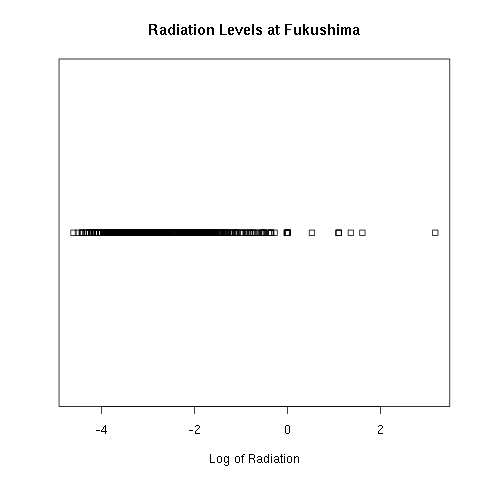
\includegraphics[width=8cm]{img/logFukushimaGamma}
  \end{center}  

\end{frame}

\begin{frame}
  \frametitle{Radiation Data}

  \begin{center}
    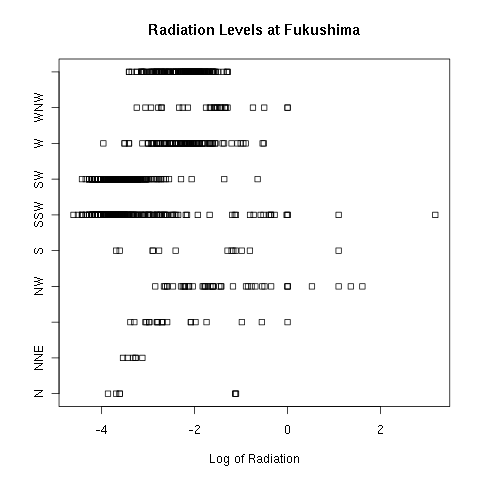
\includegraphics[width=8cm]{img/logFukushimaGammaByDirection}
  \end{center}  

\end{frame}


% LocalWords:  Clarkson pausesection hideallsubsections Cuby Webworks Webwork
% LocalWords:  ResponseCard Fukushima
